\documentclass{beamer}

\usepackage{amsthm}
\usepackage[utf8]{inputenc}
\usepackage[T1]{fontenc}
\usepackage[brazil]{babel}
\usepackage[export]{adjustbox}
\usepackage{listings}
\usepackage{fontspec}
\usepackage{color}

\definecolor{pblue}{rgb}{0.13,0.13,1}
\definecolor{pgreen}{rgb}{0,0.5,0}
\definecolor{pred}{rgb}{0.9,0,0}
\definecolor{pgrey}{rgb}{0.46,0.45,0.48}

\lstset{language=Java,
  showspaces=false,
  showtabs=false,
  breaklines=true,
  showstringspaces=false,
  breakatwhitespace=true,
  commentstyle=\color{pgreen},
  keywordstyle=\color{pblue},
  stringstyle=\color{pred},
  basicstyle=\ttfamily,
}


\usetheme{Madrid}
\usecolortheme{beetle}
\usefonttheme{professionalfonts}

\setmainfont{Oswald}

\lstset{basicstyle=\ttfamily,breaklines=true}
\beamertemplatenavigationsymbolsempty

\begin{document}

\selectlanguage{brazil}
\title[QuickSort]{QuickSort}
\author{Prof. Andrey Masiero}

\begin{frame}[plain,noframenumbering]
  \titlepage
\end{frame}

\begin{frame}[plain,noframenumbering]
  \frametitle{Agenda}
  \tableofcontents
\end{frame}

\section{QuickSort}

\begin{frame}
	\frametitle{QuickSort}
    \begin{itemize}[<+->]
        \item Assim como o MergeSort, é um algoritmo que tem base no paradigma de divisão e conquista;
        \item Só que utiliza a técnica de maneira contrária. Trabalho pesado é feito antes das chamadas recursivas;
        \item Dado uma sequência S:
        \begin{itemize}
            \item Aplica a técnica de divisão e conquista, fazendo subsequências de S;
            \item Aplica a recursão ordenando cada subsequência;
            \item Por fim, combina as subsquências ordenadas através de uma concatenação simples.
        \end{itemize}
    \end{itemize}
\end{frame}


\begin{frame}
	\frametitle{QuickSort}
    Os três passos do algoritmo:
    \begin{itemize}[<+->]
        \item Dividir: se S tiver pelo menos dois elementos, escolhe-se um elemento $x$ de S, chamado de \emph{pivô}. Uma opção é escolher $x$ como o último elemento de S. Os demais elementos de S são removidos, e colocados em três sequências:
        \begin{itemize}
            \item L: elementos de S menores que $x$;
            \item E: elementos de S iguais a $x$;
            \item G: elementos de S maiores que $x$.
        \end{itemize}
        \item Recursão: Ordena as sequências de L e G, recursivamente;
        \item Conquista: Uni os elementos de S em ordem, a partir de L, passando por E e finalizando com G.
    \end{itemize}
\end{frame}

\begin{frame}
    \frametitle{QuickSort}
    \begin{figure}
        \centering
        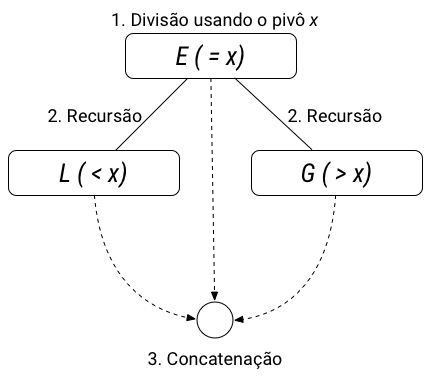
\includegraphics[scale=0.5]{images/esquema-visual.png}
        \caption{Goodrich e Tamassia, 2013}
    \end{figure}
\end{frame}

\begin{frame}
    \frametitle{QuickSort}
    \begin{itemize}[<+->]
        \item Assim como o MergeSort, o QuickSort pode ser visualizado com uma árvore binária recursiva;
        \item A altura da árvore do QuickSort é no pior caso linear;
        \item O pior caso ocorre quando a sequência consiste em n elementos distintos e já ordenada.
    \end{itemize}
\end{frame}

\begin{frame}
    \frametitle{QuickSort}
    \begin{figure}
        \centering
        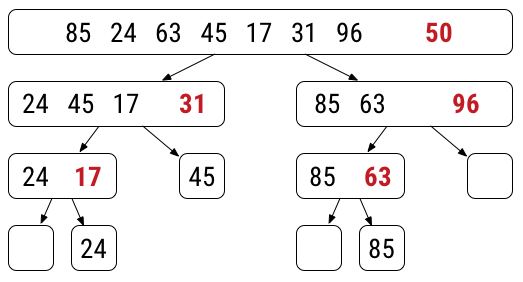
\includegraphics[scale=0.5]{images/ida.png}
        \caption{Goodrich e Tamassia, 2013}
    \end{figure}
\end{frame}

\begin{frame}
    \frametitle{QuickSort}
    \begin{figure}
        \centering
        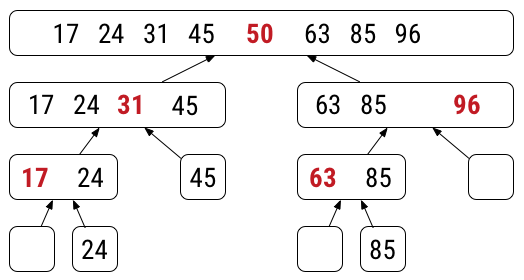
\includegraphics[scale=0.5]{images/vinda.png}
        \caption{Goodrich e Tamassia, 2013}
    \end{figure}
\end{frame}


\begin{frame}
	\frametitle{Algoritmo de Ordenação}
    \centering
    \lstinputlisting[language=Java]{src/sort.java}
\end{frame}

\begin{frame}
	\frametitle{Método Divide}
    \centering
    \lstinputlisting[language=Java]{src/divide.java}
\end{frame}

\section{Exercícios}

\begin{frame}
    \frametitle{Exercícios}

    \begin{enumerate}
        \item Implemente o QuickSort.
        \item Teste os algoritmos em um programa principal, com o seguintes vetores:
        \begin{enumerate}
            \item 42, 21, 37, 75, 98, 11, 50, 63
            \item 88, 15, 27, 55, 44, 38
            \item 12, 81, 75, 37, 47, 25, 34
            \item 48, 11, 88, 33, 57, 12, 18, 87, 54, 8
        \end{enumerate}
    \end{enumerate}
\end{frame}

\section{Referências}

\begin{frame}
    \frametitle{Referências Bibliográficas}
    \begin{enumerate}
        \item Cormen, Thomas H., Charles E. Leiserson, Ronald L. Rivest, and Clifford Stein. ``Introduction to algorithms second edition.'' (2001).
        \item Goodrich, Michael T. and Tamassia, Roberto. ``Estrutura de Dados e Algoritmos em Java.'' Porto Alegre, Ed. Bookman 5 (2013).
        \item Ascencio, Ana Fernanda Gomes, and Graziela Santos de Araújo. ``Estruturas de Dados: algoritmos, análise da complexidade e implementações em JAVA e C/C++.'' São Paulo: Perarson Prentice Halt 3 (2010).
    \end{enumerate}
\end{frame}

\end{document}
